\documentclass[a4paper]{article}

\input{style/ch_xelatex.tex}

\lstset{frame=, basicstyle={\footnotesize\ttfamily}}

\graphicspath{{images/}}
\usepackage{ctex}

%-----------------------------------------BEGIN DOC----------------------------------------
\begin{document}
\renewcommand{\contentsname}{目\ 录}
\renewcommand{\appendixname}{附录}
\renewcommand{\appendixpagename}{附录}
\renewcommand{\refname}{参考文献} 
\renewcommand{\figurename}{图}
\renewcommand{\tablename}{表}
\renewcommand{\today}{\number\year 年 \number\month 月 \number\day 日}

\title{{\Huge 个人实验报告{\large\linebreak\\}}{\Large 计算机网络实验考核\linebreak\linebreak}}
\author{\\姓\ 名: 林\ 宏\ 宇\\
学\ 号: 23320093\\
\\\\\\\\\\\\\\\\\\\\\\\\\\\\\\\\
小组 3 \\}
\date{\today}
\maketitle
\newpage

%-----------------------------------------ABSTRACT-------------------------------------
\begin{center}
{\Large\bf{摘\ 要\\}}
\end{center}

本次计算机网络期末实验以多交换机、多路由器构成的综合网络拓扑为实验对象，围绕交换机环路消除与生成树协议、VLAN 划分与 VLAN 间路由、OSPF 动态路由协议、基于时间的 ACL 访问控制以及 TCP 可靠传输等关键网络技术展开。  

在本次小组实验中，我主要负责实验一（交换机环路消除与 RSTP）、实验二（VLAN 划分与 VLAN 间路由）以及实验四（基于时间的 ACL 访问控制）的整体配置、验证与问题分析工作，同时参与实验拓扑规划、小组成员技术讨论以及实验报告的整理与撰写。  

通过本次期末综合实验，将课堂中分散学习的网络协议与配置技术进行了系统整合，不仅加深了对计算机网络体系结构的整体理解，也显著提升了在复杂网络环境下进行配置、排错与分析的工程实践能力。

\newpage
\tableofcontents
\newpage

%----------------------------------------OVERVIEW----------------------------------------
\section{实验概述}

根据课程实验总体要求，本次期末实验共划分为五个相互关联的任务模块：  
实验一为交换机环路消除与 RSTP 配置；实验二为 VLAN 划分及 VLAN 间路由；实验三为 OSPF 动态路由协议部署；实验四为基于时间的 ACL 访问控制；实验五为基于 TCP 的文件与文本传输实验。

各实验模块并非孤立完成，而是共同构成一个完整的企业级网络场景。在小组分工中，我主要承担了二层交换、VLAN 规划及网络安全控制相关实验内容，并在实验实施过程中与组员保持紧密协作，确保整体拓扑功能与实验目标的一致性。最后完成本次实验报告的撰写，和组员共同顺利完成此次实验。以下内容将围绕本人在本次实验中的具体工作与贡献进行说明。

%----------------------------------------WORK----------------------------------------
\section{本人承担的工作}

\subsection{实验拓扑理解与设备规划}

在实验开始阶段，我参与了整体网络拓扑的分析与理解工作，重点关注交换机冗余链路、VLAN 划分方案以及路由器接口角色划分等关键设计点。并和组员一起完成了此次实验总体的拓扑结构，在对拓扑结构的梳理过程中，也明确了后续各实验模块的功能与具体实验步骤。

%添加拓扑图
\begin{figure}[H]
	\centering
	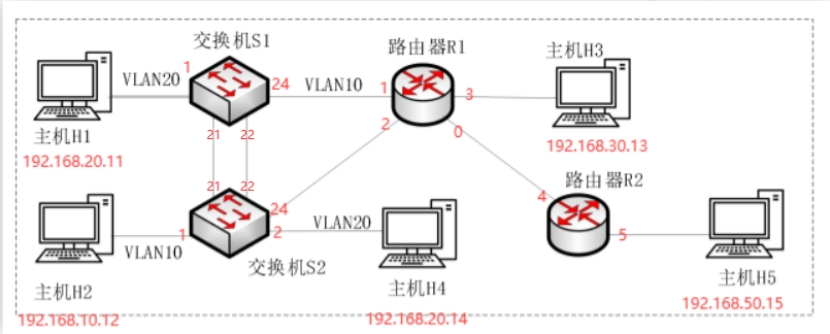
\includegraphics[width=\textwidth]{images/1.jpg}
	\caption{实验总体网络拓扑结构}
\end{figure}

\subsection{交换机环路消除与 RSTP 配置}

在实验一中，我主要负责主机和交换机的配置，并对广播风暴的产生和消除进行验证工作。根据实验报告所示拓扑，交换机之间存在冗余链路，如果未正确启用生成树协议，将导致二层网络形成环路。

\subsubsection{基础配置与环路准备}

在实验开始前，我们为主机 H1 和 H4 配置了基础 IP 地址。将 H1 配置为 192.168.20.11/24，H4 配置为 192.168.20.14/24，并禁用了校园网卡以避免干扰。通过 Telnet 远程登录交换机 S1（172.16.17.201）和 S2（172.16.17.202），执行 \texttt{undo stp enable} 命令手动关闭默认开启的 STP 功能。这一操作为后续环路制造和现象观察奠定了基础。

\subsubsection{基准测试与环路制造}

关闭 STP 功能后，我们在制造环路之前进行了基准测试。此时 S1 与 S2 之间仅有一条物理链路（GE0/0/22 ↔ GE1/0/22），网络中不存在环路。通过在 H1 和 H4 上执行 \texttt{ping} 命令，验证了单链路情况下的正常通信状态，为后续对比分析提供参考。

\begin{figure}[H]
    \centering
    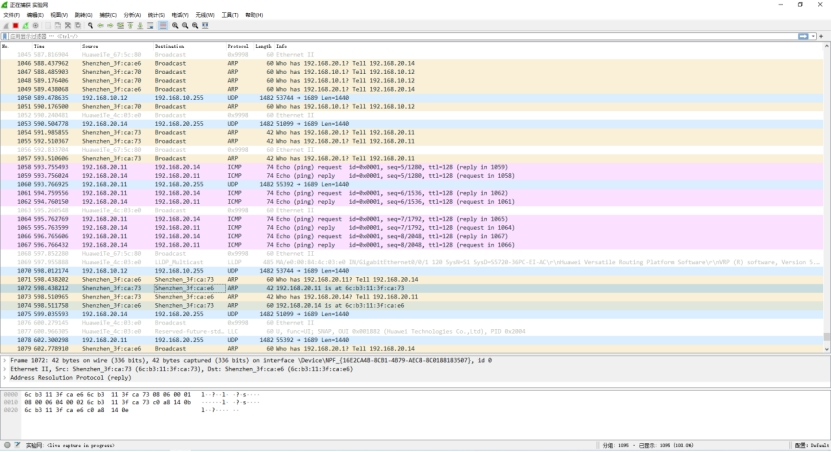
\includegraphics[width=\textwidth]{images/7.jpg}
    \caption{Wireshark 捕获 H1 ping H4 的 ICMP 流量}
\end{figure}

同时验证不同的vlan下 H1 与 H2 此时无法进行正常通信，为同一vlan下的 H1 和 H4 正常通信做对比，同时为后续的 vlan 间路由配置奠定基础

接下来，启动 Wireshark 抓包工具，并开始持续向 H4 发送 ping 请求。在此过程中，手动连接 S1 与 S2 之间的第二条冗余链路（S1 GE0/0/21 ↔ S2 GE1/0/21），从而在二层网络中制造了物理环路。

\subsubsection{广播风暴现象观察与分析}

连接第二条链路后，网络状态急剧恶化。H1 原本能够 ping 通的 H4 立即变为"请求超时"，交换机 S1 和 S2 的端口指示灯开始异常高频闪烁，表明设备正在处理大量流量。

通过 Wireshark 抓包分析，我观察到网络中充斥着大量的 ARP 和 UDP 广播报文，短时间内捕获的数据包数量达到上千万级。这是典型的广播风暴现象：一个广播帧（如 ARP 请求）进入环路后，被两台交换机在环路链路上持续复制和转发，迅速耗尽了所有可用的网络带宽和设备处理能力，导致正常通信（如 ICMP）完全瘫痪。

\begin{figure}[H]
    \centering
    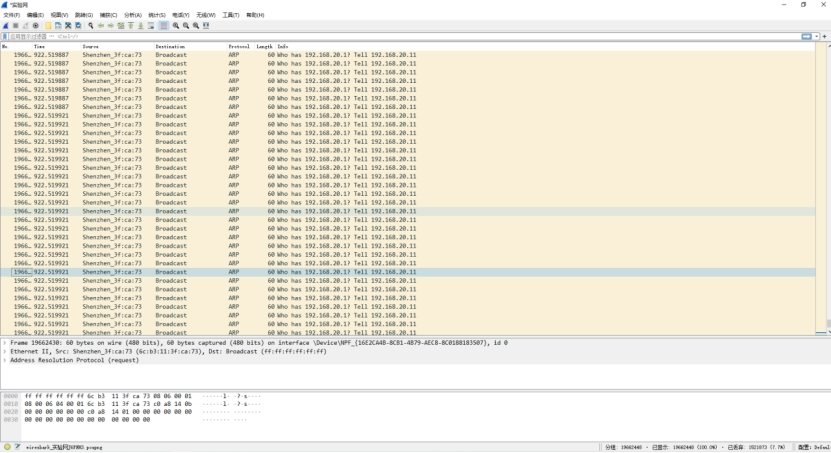
\includegraphics[width=\textwidth]{images/12.jpg}
    \caption{网络风暴中的 ARP 广播报文}
\end{figure}

\subsubsection{RSTP 部署与状态验证}

为解决广播风暴问题，我们采用快速生成树协议（RSTP）作为解决方案。在 S1 和 S2 上重新启用生成树功能，并将其模式设置为 \texttt{rstp}：

\begin{lstlisting}
system-view
stp mode rstp
stp enable
quit
save
\end{lstlisting}

配置完成后，再次连接 S1 与 S2 之间的两条链路，并等待约30秒以便 RSTP 协议完成收敛。随后登录两台交换机，使用 \texttt{display stp brief} 命令查看生成树状态。

\subsubsection{RSTP 工作效果分析}

通过 \texttt{display stp brief} 输出结果，我观察到 RSTP 的工作效果：在 S2 上，端口 GigabitEthernet1/0/22 的角色（Role）为 \texttt{ALTE}（Alternate Port），状态（STP State）为 \texttt{DISCARDING}。这表明 RSTP 协议成功识别出这是一个冗余端口，并将其置于阻塞状态，从而打破了物理环路，形成了一个无环的逻辑树状拓扑。

最终的连通性测试验证了解决方案的有效性：即使在物理上存在环路，H1 和 H4 之间的通信也完全恢复正常，网络风暴问题得到彻底解决，充分验证了 RSTP 快速收敛与环路消除的核心功能。

\subsection{VLAN 划分与 VLAN 间路由配置}

在实验二中，我主要负责交换机 VLAN 配置、Trunk 链路设置以及路由器 R1 上 VLAN 间路由的配置与排错工作。

\subsubsection{设计思路与基础配置}

根据主实验报告的 VLAN 规划方案，需要将主机 H1、H4 划入 VLAN 20，主机 H2 划入 VLAN 10。我首先为新增主机 H2 配置了静态 IP 地址（192.168.10.12/24）。

在配置开始之前，需要禁用校园网卡以防止对实验网造成印象。

在配置 VLAN 前，我们进行了初始连通性测试作为基准。在默认的二层交换环境下，H1 (192.168.20.11) 与 H4 (192.168.20.14) 能够正常双向通信，因为它们在同一个 IP 子网中；而 H1/H4 与 H2 (192.168.10.12) 之间的跨网段通信全部失败，这暴露了缺乏三层路由设备的问题。

\subsubsection{交换机 VLAN 与 Trunk 详细配置}

在交换机 S1 和 S2 上进行了系统的 VLAN 配置：

S1 配置：
\begin{lstlisting}
vlan batch 10 20
interface GigabitEthernet0/0/1
 port link-type access
 port default vlan 20    # H1端口
interface GigabitEthernet0/0/24
 port link-type access  
 port default vlan 10    # 连接R1端口
interface GigabitEthernet0/0/21
 port link-type trunk
 port trunk allow-pass vlan all  # 连接S2的冗余链路
\end{lstlisting}

S2 配置：
\begin{lstlisting}
vlan batch 10 20
interface GigabitEthernet0/0/1
 port link-type access
 port default vlan 10    # H2端口
interface GigabitEthernet0/0/2  
 port link-type access
 port default vlan 20    # H4端口
interface GigabitEthernet1/0/24
 port link-type trunk
 port trunk allow-pass vlan all  # 连接R1端口
\end{lstlisting}

\subsubsection{路由器网关配置与单臂路由}

在路由器 R1 上，采用了混合配置策略：将连接 S1 的物理接口 GE0/0/1 直接配置为 VLAN 10 的网关（192.168.10.1），将连接 S2 的 GE0/0/2 启用为物理接口，并在其上创建绑定 VLAN 20 的逻辑子接口：

\begin{lstlisting}
interface GigabitEthernet0/0/1
 ip address 192.168.10.1 24  # VLAN 10网关
interface GigabitEthernet0/0/2
 undo shutdown
interface GigabitEthernet0/0/2.20
 dot1q termination vid 20
 ip address 192.168.20.1 24  # VLAN 20网关
 arp broadcast enable
\end{lstlisting}

这种设计确保了每个 VLAN 都有唯一且专用的网关，避免了地址冲突。

\subsubsection{连通性验证与路径分析}

VLAN 内通信：H1 ping H4 (均属 VLAN 20) 一跳直达，纯二层转发

\begin{figure}[H]
    \centering
    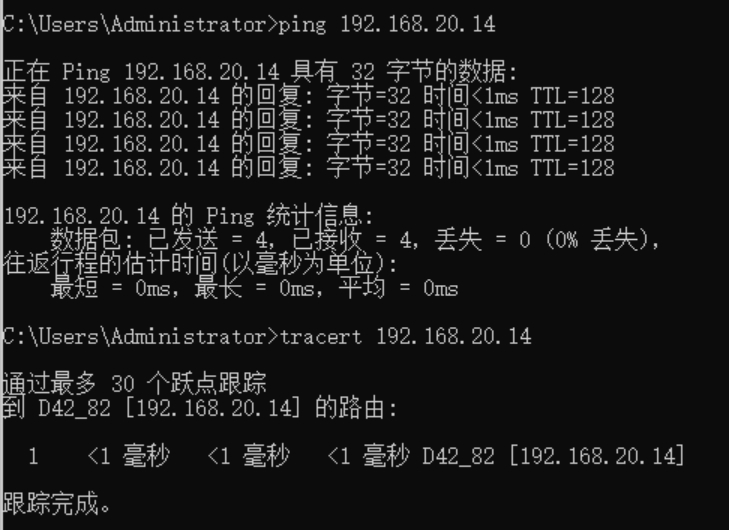
\includegraphics[width=0.6\textwidth]{images/28.jpg}
    \caption{H1 ping \& tracert H4}
\end{figure}

VLAN 间通信：H1 ping H2, H2 ping H4 等跨 VLAN 通信均成功，\texttt{tracert} 显示经过两跳：第一跳为对应的 VLAN 网关，第二跳为目标主机

\begin{figure}[H]
    \centering
    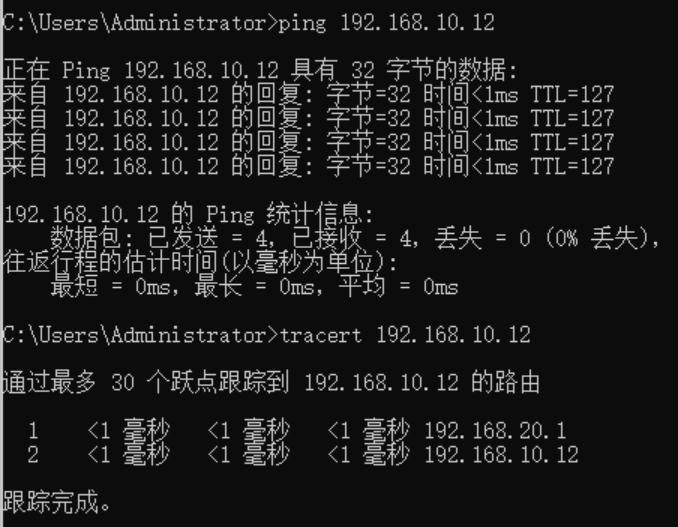
\includegraphics[width=0.48\textwidth]{images/29.jpg}\hfill
    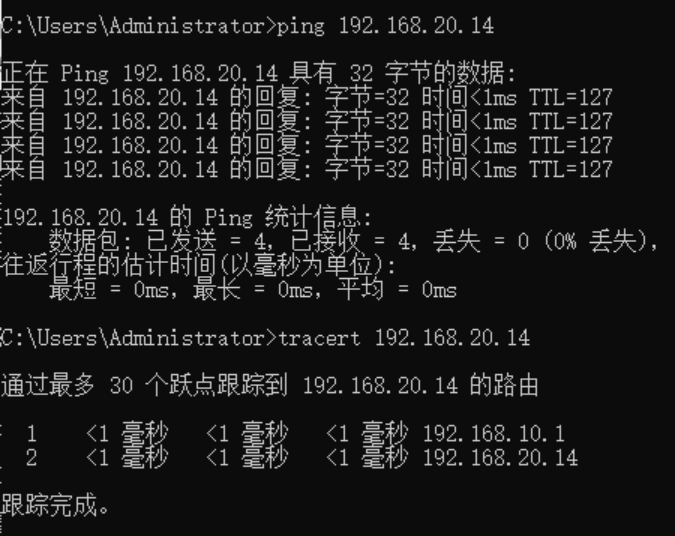
\includegraphics[width=0.48\textwidth]{images/31.jpg}
    \caption{左：H1 ping \& tracert H2；右：H2 ping \& tracert H4}
\end{figure}

通过同一 Vlan 下和不同 Vlan 下的主机连通性测试，验证了 VLAN 划分实现了逻辑隔离，同时路由器 R1 作为三层网关成功实现了 VLAN 间的可控互通。

\subsection{基于时间的 ACL 访问控制}

在实验四中，我主要负责基于时间的 ACL 规则设计、配置与验证，实现复杂的分时段访问控制策略。

\subsubsection{ACL 设计思路与策略规划}

根据实验要求，需要实现以下复杂的访问控制策略：
\begin{itemize}
\item \textbf{08:00-11:00}：H1 与 H5 互访，H2 与 H3 互访，但禁止 H1 与 H3、H2 与 H5
\item \textbf{14:00-17:00}：H1 与 H3 互访，H2 与 H5 互访，但禁止 H1 与 H5、H2 与 H3  
\item \textbf{其余时段}：禁止 H1 与 (H3,H5) 互通，禁止 H2 与 (H3,H5) 互通
\item \textbf{全时段不受限}：H4 与任意主机互通，H3 与 H5 互通，H1 与 H2 互通
\end{itemize}

我们采用了"优先放行特权，再按时段匹配，最后全部禁止"的设计思路，并选择在 R1 的流量入口（GE0/0/1 和 GE0/0/2.20）应用 ACL 实现集中管控。

\subsubsection{ACL 规则}
    \begin{itemize}
        \item \textbf{10 \& 11}：允许H4与全网任意主机双向互通。
        \item \textbf{20 \& 21}：H3与H5的通信全时段不受限制。
        \item \textbf{30 \& 31}：允许VLAN 10与VLAN 20之间双向互访。
        \item \textbf{110 \& 111}：在上午时段允许H1与H5之间双向互访。
        \item \textbf{120 \& 121}：在上午时段允许H2与H3之间双向互访。
        \item \textbf{112 \& 113}：在上午时段拒绝H2与H5之间的双向互访。
        \item \textbf{210 \& 211}：在下午时段允许H1与H3之间双向互访。
        \item \textbf{220 \& 221}：在下午时段允许H2与H5之间双向互访。
        \item \textbf{212 \& 213}：在下午时段拒绝H1与H5之间的双向互访。
        \item \textbf{222 \& 223}：在下午时段拒绝H2与H3之间的双向互访。
        \item \textbf{500 \& 501}：在其余所有时段禁止H1与H3,H1与H5之间的双向互访。
        \item \textbf{502 \& 503}：在其余所有时段禁止H2与H3,H2与H5之间的双向互访。
    \end{itemize}

每一对主机通信都配置了双向规则，确保无论谁发起连接都能被正确匹配和处理。

\subsubsection{分时段验证与结果分析}

我通过手动修改 R1 系统时间的方式，分别在 10:00（上午）、15:00（下午）、20:00（其余时段）进行了全面测试：

\textbf{上午时段测试（10:00）}：
\begin{itemize}
    \item H1 与 H5 互访
    \item H2 与 H3 互访
    \item H1 与 H3 禁止互访
    \item H2 与 H5 禁止互访
    \item H4 与任意主机互通
    \item H3 与 H5 不受限互通
    \item H1 与 H2 不受限互通
\end{itemize}

\textbf{下午时段测试（15:00）}：
\begin{itemize}
    \item H1 与 H3 互访
    \item H2 与 H5 互访
    \item H1 与 H5 禁止互访
    \item H2 与 H3 禁止互访
    \item H4 与 任意主机 互通
    \item H3 与 H5 不受限互通
    \item H1 与 H2 不受限互通
\end{itemize}

\textbf{其余时段测试（20:00）}：
\begin{itemize}
    \item H1 与 H3 禁止互访
    \item H1 与 H5 禁止互访
    \item H2 与 H3 禁止互访
    \item H2 与 H5 禁止互访
    \item H4 与 任意主机 互通
    \item H3 与 H5 不受限互通
    \item H1 与 H2 不受限互通
\end{itemize}

所有测试结果均与预期策略完全一致，成功实现了基于时间的复杂双向访问控制。

\subsection{实验报告整理与协作}

在实验报告阶段，我使用 Overleaf 平台与组员协作完成主实验报告的整理与排版工作，负责部分配置命令、抓包现象及实验分析内容的撰写与校对，保证实验报告整体结构清晰、表述规范。

%--------------------------------problem and solution----------------------------------
\section{遇到的困难与解决方法}

在整个实验过程中，我遇到了多个技术难点和配置问题，通过系统性的分析和解决，最终成功完成了各项实验任务。

\subsection{初期未能正确观察到网络风暴}

在实验一的初始阶段，我按照实验指导连接了 S1 和 S2 之间的两条物理链路，但初次测试时网络依然能够正常工作，没有出现预期的广播风暴现象。这与实验手册中的描述不符，让我一度怀疑实验设计是否正确。

\textbf{问题分析：}

通过检查交换机配置，我发现了问题的根源：华为交换机在出厂默认情况下是启用 STP 功能的。这意味着即使我连接了多条链路，系统依然会自动阻塞冗余链路以防止环路的产生。

\textbf{解决方法：}
\begin{enumerate}
\item 通过 Telnet 登录到 S1 和 S2，执行 \texttt{display stp brief} 命令确认 STP 状态
\item 在两台交换机上依次执行 \texttt{undo stp enable} 命令手动关闭 STP 功能
\item 重新连接第二条链路，这次成功观察到了明显的广播风暴现象
\item 使用 Wireshark 抓包工具记录并分析了 ARP 请求和 UDP 广播帧的循环放大过程
\end{enumerate}

\subsection{VLAN 间通信初期失败}

在完成基本 VLAN 划分之前，我发现同一 VLAN 下 H1 与 H4 之间仍然无法通信。

\textbf{问题分析：}

因为 H1 与 H4 按照拓扑图连接在同一交换机上，不需要进行信息配置，只需要保证物理接线正确既可以进行通信，通过检查交换机物理接口，发现由于接线太多导致出现接口连接错误的情况，使得无法进行正常通信。

\textbf{解决方法：}
\begin{enumerate}
\item 重新完成 H1 与 H4 的物理连接，确保它们正确连接到 S1 的端口上
\item 再次测试 H1 与 H4 之间的连通性，成功实现 ping 通
\item 同时结合拓扑图检查其他的物理接线，确保所有主机均连接到正确的交换机端口
\end{enumerate}

\subsection{部分时间段的禁止通信规则未生效}

在完成 ACL 初始配置后，我发现在某些时间段内，一些应该被禁止的通信仍然能够成功。例如，在上午 10:00 时段，H1 应该无法 ping 通 H3，但实际测试中却能够 ping 通。

\textbf{问题诊断与分析：}
\begin{enumerate}
\item 检查 ACL 规则顺序：通过 \texttt{display acl 3000} 查看所有规则
\item 检查时间段匹配：通过 \texttt{display time-range} 确认时间配置
\item 检查规则命中情况：通过 \texttt{display acl 3000 verbose} 查看规则使用统计
\item 发现问题出现在规则匹配的逻辑中。由于 ACL 规则设计不够完美，忽视了部分主机之间的通信权限。
\end{enumerate}

\textbf{解决方案：}
\begin{enumerate}
\item 重新整理 ACL 规则的优先级策略，采用更细粒度的匹配
\item 用主机精确匹配替代网段匹配，避免意外覆盖
\end{enumerate}

\subsection{设备故障问题}

在实验过程中，我们遇到了 3 组原定设备出现故障的问题，需要使用 15 组和 17 组的设备进行替代。这导致了一些配置参数和 IP 地址规划的调整。

\textbf{解决策略：}
\begin{enumerate}
\item 重新规划设备对应关系和 IP 地址分配
\item 验证不同设备的命令语法差异，特别是路由器和交换机的配置命令
\item 建立设备配置对照表，确保所有组员使用统一的参考标准
\end{enumerate}

%----------------------------------------SUMMARY----------------------------------------
\section{体会与总结}

本学期的计算机网络课程从链路层到应用层系统展开，期末综合实验将课堂知识与实际设备配置紧密结合。我在环路控制、VLAN 规划、三层路由、ACL 安全等环节中，真实体验了协议原理如何落地为工程配置，既复盘了课上的关键概念，也体会到参数、时延、收敛等细节对网络稳定性的影响。

在本次实验中，从制造环路观察广播风暴到借助 RSTP 收敛消除环路，再到单臂/物理网关混合方案实现 VLAN 间路由，以及基于时间的 ACL 精细化管控，我对“理论—配置—验证—排错”的完整闭环有了更深的认识。抓包、tracert、显示命令等手段帮助我定位问题、验证假设，也培养了结构化排障思维。

小组协作是本次顺利完成的关键。我们在拓扑规划、接口分工、配置复核、测试记录等环节保持高频沟通，遇到设备故障、接口冲突时互相支援、快速调整，确保整体进度和一致性。协同写作报告的过程也提醒我及时记录、标准命名的重要性。

感谢任课老师与助教在课堂与实验中提供的指导和反馈，也感谢组员们的耐心讨论与互助支持。通过这次综合实践，我不仅巩固了计算机网络的核心知识，更提升了在真实场景中团队合作与工程落地的能力。

\end{document}
